\documentclass[10pt]{beamer}

\newcommand{\lectnum}{L07}
\newcommand{\lecttitle}{Regresssion and Classification Trees}

\usepackage{amsmath, amssymb, graphicx}
\usepackage[]{algorithm2e}
\usepackage{pdfpages}
\usepackage[british]{babel}

\hypersetup{colorlinks,linkcolor=,urlcolor=blue}
\newenvironment{titledslide}[1]{\begin{frame}\frametitle{#1}}{\end{frame}}

\mode<presentation>{\setbeamercovered{transparent}}

\setbeamertemplate{sidebar right}{}
\setbeamertemplate{footline}{%
\hfill\usebeamertemplate***{navigation symbols}
\hspace{0.4cm}\lectnum: \insertframenumber{}/\inserttotalframenumber \hspace*{0.4cm}}

\author{James Cussens}

\title{COMS30035, Machine learning:\\ \vspace{5pt} \lecttitle}

\institute{School of Computer Science\\University of Bristol}

\begin{document}
%%%%%%%%%%%%%%%%%%%%%%%%%%%%%%%%%%%%%%%%%%%%%%%%%%%%%%%%%%%%%%%%%%%%%%

\begin{frame}
  \titlepage
\end{frame}

%%%%%%%%%%%%%%%%%%%%%%%%%%%%%%%%%%%%%%%%%%%%%%%%%%%%%%%%%%%%%%%%%%%%%%


%%%%%%%%%%%%%%%%%%%%%%%%%%%%%%%%%%%%%%%%%%%%%%%%%%%%%%%%%%%%%%%%%%%%%%
\begin{titledslide}{Acknowledgement}

  \begin{itemize}
  \item These slides are adapted from ones originally created by Edwin Simpson. 
  \end{itemize}
  
\end{titledslide}
%%%%%%%%%%%%%%%%%%%%%%%%%%%%%%%%%%%%%%%%%%%%%%%%%%%%%%%%%%%%%%%%%%%%%%

% \begin{frame}
% \frametitle{Decision Trees}

% \begin{tikzpicture}
% \node[draw] at (8,1.3) {Weight $>$ 5kg};
% \draw(8,1) -- (6,0);
% \node[draw=none] at (6.4,0.5) {true};
% \draw(8,1) -- (10,0);
% \node[draw=none] at (9.6,0.5) {false};

% \node[draw] at (6,-0.3) {A: Dog};

% \node[draw] at (10,-0.3) {Height $<$ 15cm};
% \draw(10, -0.6) -- (8,-1.6);
% \draw(10, -0.6) -- (12,-1.6);
% \node[draw=none] at (8.3,-1.1){false};
% \node[draw=none] at (11.6,-1.1){true};
% \node[draw] at (8,-1.9){B: Dog};
% \node[draw] at (12,-1.9){C: Cat};

% \draw[style={very thick, ->, >=stealth'}](13,-2) -- (13,1.5);
% \draw[style={very thick, ->, >=stealth'}](13,-2) -- (17,-2);
% \draw(15,-2) -- (15,1.5);
% \draw(13,0) -- (15,0);
% \node[draw=none] at (15,-2.4){weight};
% \node[draw=none] at (12.4,1.2){height};

% \node[draw=none] at (16,0){A: Dog};
% \node[draw=none] at (14,1){B: Dog};
% \node[draw=none] at (14,-1){C: Cat};

% \end{tikzpicture}

% \end{frame}

\begin{frame}
\frametitle{Decision Trees}

A Decision Tree is a tree-structured predictive model where:
\begin{itemize}
\item Each internal node represents a decision test on a feature (e.g., Is salary $>50k$?).
\item Each branch represents the outcome of the test (e.g., yes/no).
\item Each leaf node represents a predicted class label (for classification) or a numerical value (for regression).
\end{itemize}

\center
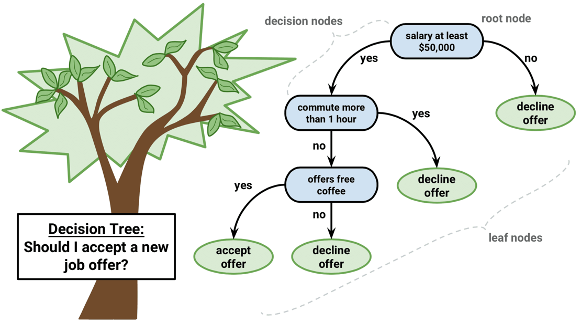
\includegraphics[width=0.8\textwidth]{figures/pic1.png}

\end{frame}

\begin{frame}
\frametitle{Decision Trees as Partitioning Input Space}
\begin{itemize}
\item One model is responsible for assigning a decision for each region
of input space;
\item The correct model for an input $\bs x$ 
is chosen by traversing the binary decision tree, following
 the path from the top to a leaf.
\item Leaf node is responsible for assigning a decision, such as a:
	\begin{itemize}
	\item Class label;
	\item Probability distribution over class labels;
	\item Scalar value (for regression tasks).
	\end{itemize}
%\item Mixtures of Experts assign points to regions of input space with soft borders by weighting models probabilistically.
\end{itemize}
\end{frame}

\begin{frame}
\frametitle{Learning the Tree Structure}
\begin{itemize}
\uncover<2->{\item Which input variable to use at each node?}
\uncover<3->{\item Which attributes will be used to split at each node? How to determine the threshold?}
\uncover<4->{\item Classification and Regression Trees (CART): one of many possible learning algorithms
\item Objective: greedily minimise the error 
\begin{itemize}
\item Regression: sum-of-squares
\item Classification: cross-entropy as used in neural networks or Gini impurity
\end{itemize}}
\end{itemize}
\end{frame}


\begin{frame}
\frametitle{Learning the Tree Structure}
\begin{itemize}
\item Number of possible solutions grows combinatorially with the number of input variables
\item Greedy algorithm: add nodes one-at-a-time, choosing the best split at each point
\begin{enumerate}
\uncover<2->{\item Start from the root node}
\uncover<3->{\item Run \emph{exhaustive search} over each possible variable and threshold for a new node. For each variable and threshold:
\begin{itemize}
\item Compute average of the target variable for each leaf of the proposed node
\item Compute the error if we stop adding nodes here
\end{itemize}}
\uncover<4->{\item Choose the variable \& threshold that minimise the error}
\uncover<5->{\item Add a new node for the chosen variable and threshold.}
\uncover<6->{\item Repeat step 2 until there are only $n$ data points associated with each leaf node.}
\uncover<7->{\item Prune back the tree to remove branches that do not reduce error by more than a small tolerance value, $\epsilon$.}
\end{enumerate}
\end{itemize}
\end{frame}


\begin{frame}
\frametitle{Attribute Selection in CART}

\begin{itemize}
\item For Classification Trees:

Gini Impurity (for Classification):
\begin{equation}
    Gini(D) = 1 - \sum_{i=1}^{C} p_i^2
\end{equation}

Information Gain (optional): 
\begin{equation}
IG(D, A) = Entropy(D) - \sum_{v \in Splits} \frac{|D_v|}{|D|} \, Entropy(D_v)
\end{equation}

\item For Regression Trees:
\begin{equation}
    MSE(D) = \frac{1}{|D|} \sum_{i=1}^{|D|} (y_i - \bar{y})^2
\end{equation}

\end{itemize}

\end{frame}


\begin{frame}
\frametitle{Example of Information Gain Calculation}
\centering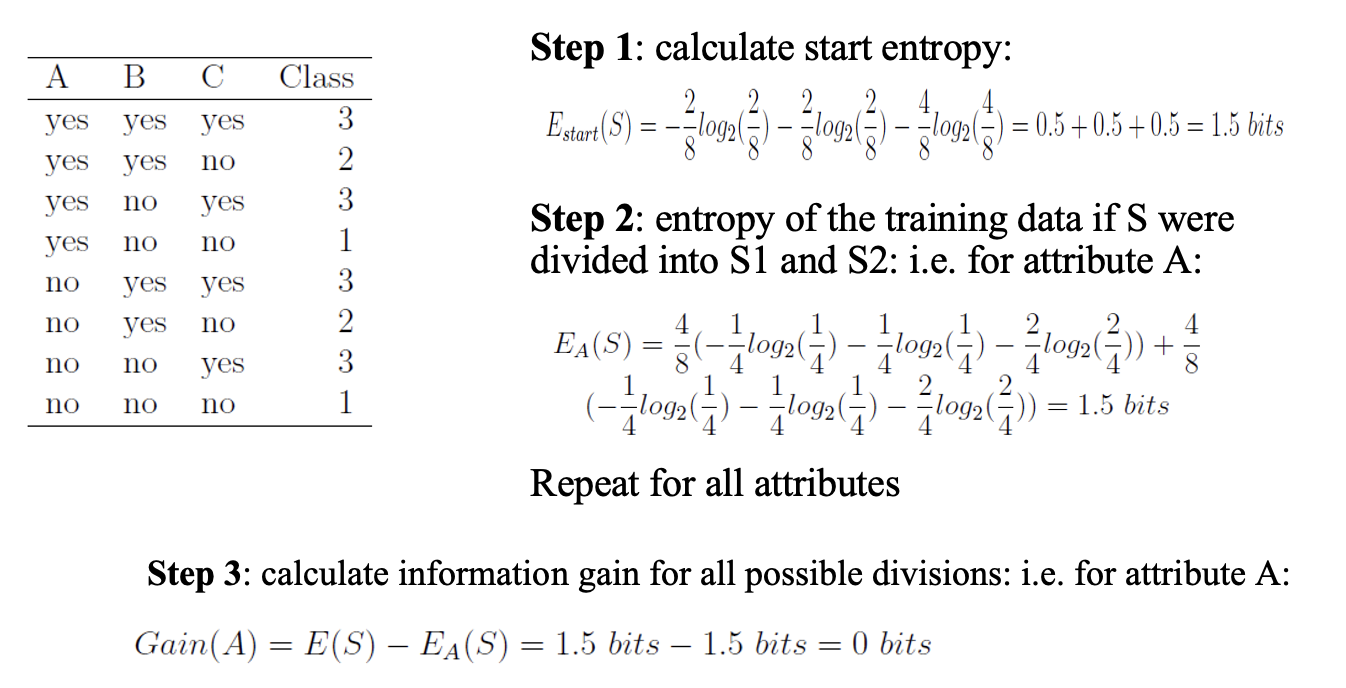
\includegraphics[width=1\textwidth]{figures/pic2.png}
\end{frame}


\begin{frame}
\frametitle{Example of Information Gain Calculation}
\centering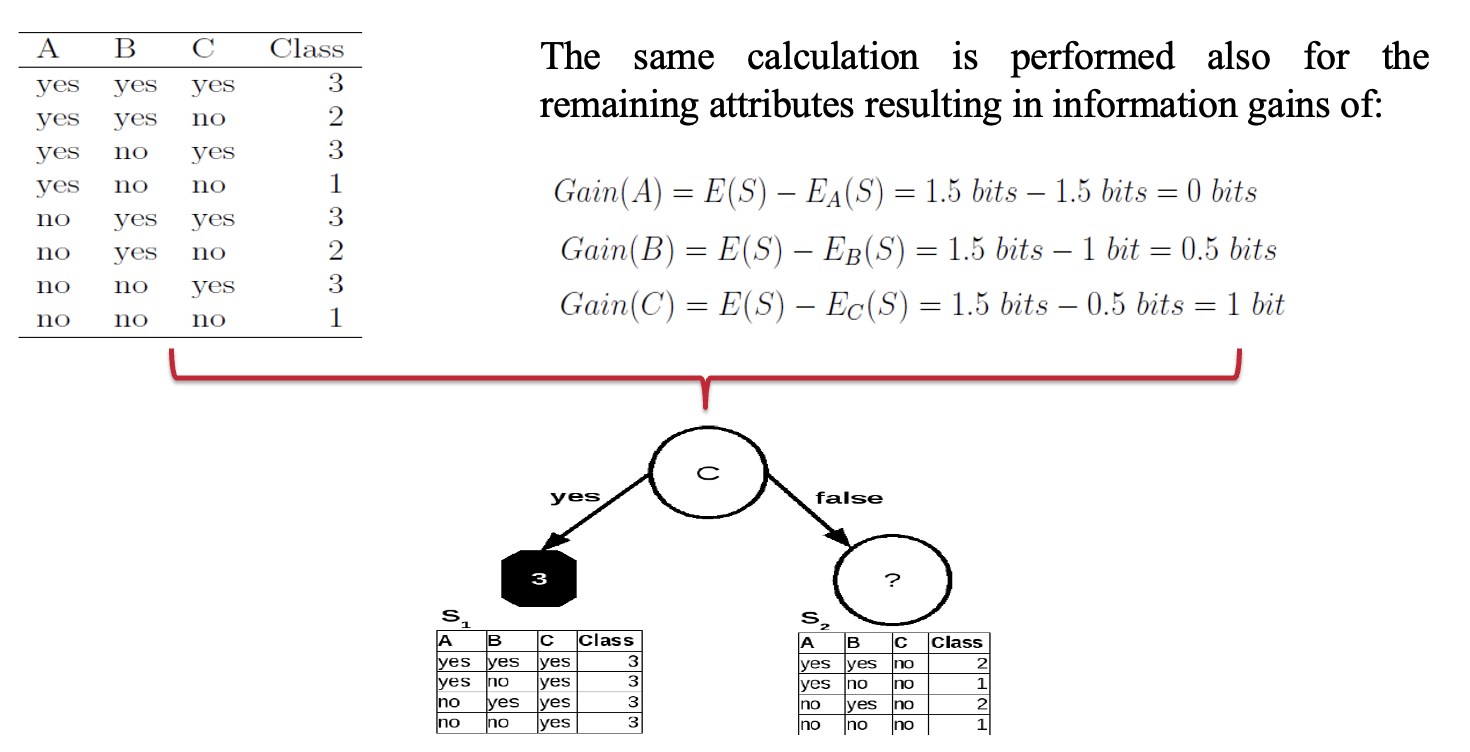
\includegraphics[width=1\textwidth]{figures/pic3.png}
\end{frame}

\begin{frame}{Stopping Criteria in Decision Trees}
\begin{itemize}
  \item Growing a tree without limits often leads to \textbf{overfitting}.
  \item We need \textbf{stopping criteria} to decide when to stop splitting:
  \begin{itemize}
    \item Maximum tree depth reached;
    \item Minimum number of samples in a leaf node;
    \item Minimum number of samples required to split a node;
    \item Impurity (e.g.\ Gini, entropy, MSE) below a threshold;
    \item No further information gain from any split.
  \end{itemize}
  \item These rules help balance \textbf{model complexity} and \textbf{generalization}.
\end{itemize}
\end{frame}


\begin{frame}
\frametitle{Pruning}

\begin{itemize}
\item Balance residual training-set error against model complexity
\item Start with a tree $T_0$
\uncover<2->{\item Consider pruning each node in $T_0$ by combining the branches to obtain tree $T$}
\uncover<3->{\item Compute a criterion $C(T) = \sum_{\tau=1}^{|T|} e_{\tau}(T) + \lambda | T | $ 
}
% C is criterion
% e is error
% lambda is the tradeoff between tree size and error
\uncover<4->{\item If $C(T) \leq C(T_0)$ keep the pruned tree, else reinstate the pruned node.}
\end{itemize}

\end{frame}


\begin{frame}
\frametitle{Interpretability}

\begin{columns}
\column{0.6\textwidth}
\begin{itemize}
\item The sequence of decisions is often easier to interpret than other methods (think of neural networks);
\item However, sometimes small changes to the dataset cause big changes to the tree;
\item If the optimal decision boundary is not aligned with the axes of an input variable, we need a lot of splits. % a combination of features needed
\end{itemize}

\vspace{10pt}
\centering
\begin{tikzpicture}
\draw[style={very thick, ->, >=stealth'}](13,0) -- (13,1.5);
\draw[style={very thick, ->, >=stealth'}](13,0) -- (17,0);
\draw[style={thick},blue](13,0) -- (17,1.5);

\draw(13,0.2) -- (14,0.2);
\draw(13,0.55) -- (17,0.55);
\draw(15,0.9) -- (17,0.9);
\draw(16,1.3) -- (17,1.3);

\draw(14,0) -- (14,0.55);
\draw(15,0.55) -- (15,1.5);
\draw(16,0.9) -- (16,1.5);

\node[draw=none] at (15,-0.4){\scriptsize feature 1};
\node[draw=none] at (12.4,1.2){\scriptsize feature 2};

\node[draw=none] at (14,1){A};
\node[draw=none] at (16,0.5){B};
\end{tikzpicture}

\column{0.5\textwidth}
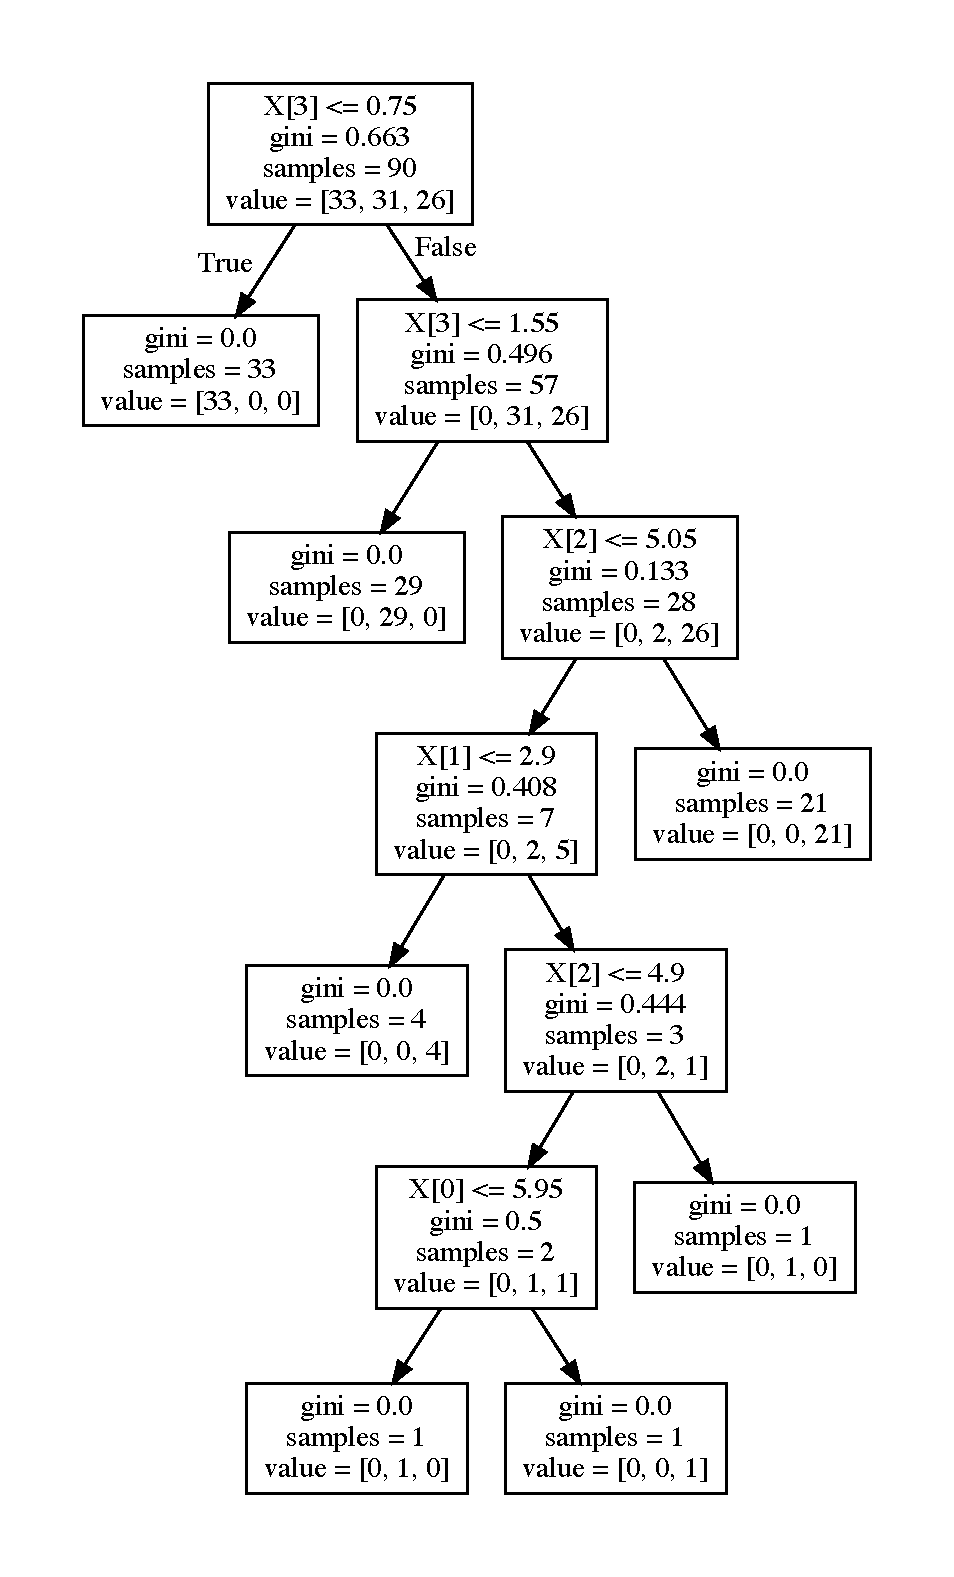
\includegraphics[width=\textwidth]{../figures/iris_decision_tree}
\end{columns}
\end{frame}



\begin{frame}{Pros and Cons of CART}
\begin{columns}[T] % align columns at the top
  \begin{column}{0.48\textwidth}
    \textbf{Pros}
    \begin{itemize}
      \item Easy to interpret and visualize
      \item Handles both classification and regression
      \item Non-parametric (no strong assumptions)
      \item Works with numerical and categorical features
      \item Captures nonlinear relationships
      \item Robust to scaling of features
    \end{itemize}
  \end{column}
  \begin{column}{0.48\textwidth}
    \textbf{Cons}
    \begin{itemize}
      \item Prone to overfitting (needs pruning)
      \item High variance (unstable to small data changes)
      \item Only axis-aligned splits
      \item Biased toward features with many split points
      \item Single tree is often less accurate than ensembles
      \item Regression outputs are piecewise constant
    \end{itemize}
  \end{column}
\end{columns}
\end{frame}


\begin{frame}{Ensemble Methods}


\begin{itemize}
  \item \textbf{Bagging (Bootstrap Aggregating)} \\
        Train multiple trees on bootstrapped samples; average or vote. 
        \textit{(Reduces variance).}
  \vspace{1pt}
  \item \textbf{Random Forests} \\
        Extension of Bagging with random feature subsets at splits. 
        \textit{(Stable, accurate).}
  \vspace{1pt}
  \item \textbf{Boosting (AdaBoost, Gradient Boosting, XGBoost)} \\
        Sequentially build trees, focusing on correcting errors (reduces bias). 
        \textit{(High accuracy).}
\end{itemize}

\centering
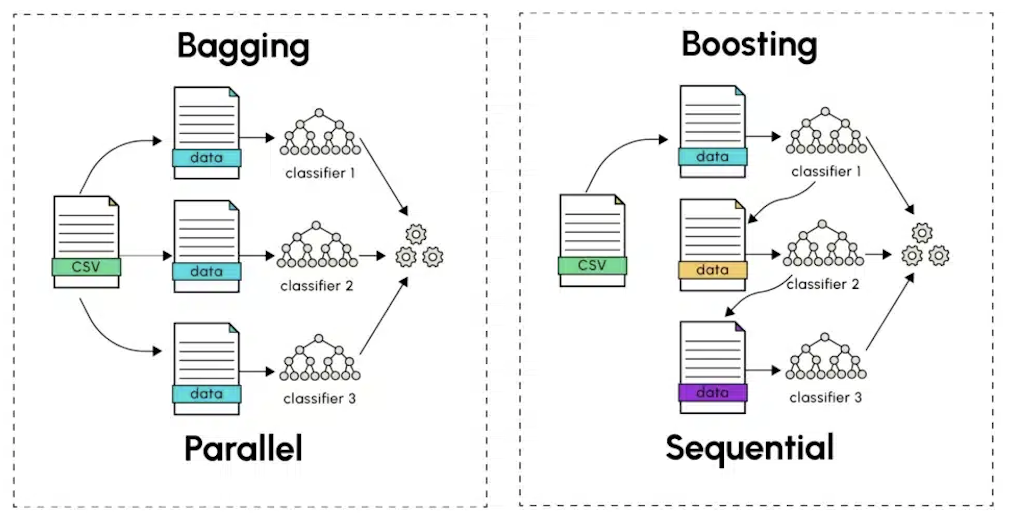
\includegraphics[width=10cm,height=3cm]{figures/pic4.png}

https://datascientest.com/en/bagging-vs-boosting

\end{frame}



%%%%%%%%%%%%%%%%%%%%%%%%%%%%%%%%%%%%%%%%%%%%%%%%%%%%%%%%%%%%%%%%%%%%%%
\begin{titledslide}{Reading}

  There is typo on p.\ 666 of Bishop where a minus sign has gone
  missing. Equation (14.32) should be:
  \[
    Q_{\tau}(T) = -\sum_{k=1}^{K}p_{\tau k} \ln p_{\tau k} 
  \]
  
  \begin{itemize}
  \item Bishop \S14.4. 
  \item Murphy \S18.1
  \end{itemize}
  
  
\end{titledslide}
%%%%%%%%%%%%%%%%%%%%%%%%%%%%%%%%%%%%%%%%%%%%%%%%%%%%%%%%%%%%%%%%%%%%%%
\begin{titledslide}{Problems and quizzes}

  \begin{itemize}
  \item Bishop Exercise 14.10
  \item Bishop Exercise 14.11 (don't forget about the typo!)
  \item Quizzes:
    \begin{itemize}
    \item Week~3: Trees
    \end{itemize}
  \end{itemize}
  
\end{titledslide}
%%%%%%%%%%%%%%%%%%%%%%%%%%%%%%%%%%%%%%%%%%%%%%%%%%%%%%%%%%%%%%%%%%%%%%

\end{document}
